%% 计划完全使用LaTeX来完成@!
%%
%% This aims to be written by LaTeX totally, not XeTex
%
% file:///C:/Users/lenovo/Desktop/let'stalkenglish/Charlotte's%20Web.pdf
%%
\documentclass[a4paper, oneside]{book}
\author{E.B. White}
\title{Charlotte's Web}

\usepackage{geometry}
\usepackage{graphicx}
\usepackage[T1]{fontenc}
\usepackage{tikz}
\usepackage{tkz-base}
\usetikzlibrary{calc}
\usetikzlibrary{arrows,shapes,trees,calc,automata,positioning, fit} 
\usetikzlibrary{calendar}
\usetikzlibrary{backgrounds}
\usetikzlibrary{angles}
\usetikzlibrary{graphs}
\usepackage[framemethod=tikz]{mdframed}
\usepackage{tipa}
\usepackage{titletoc}
 
\titlecontents{chapter}[1.5em]
   {}
   {\contentslabel{2.5em}}%change the argument to obtain the 
                          %desired spacing
   {\vspace*{2.3em}}
   {\titlerule*[1pc]{.}\contentspage}
   

   

%%
%%下面的是使用罗马数字方式来标志Chapter数值
\newcommand{\ZeroRoman}[1]{% 0 + \Roman
  \ifcase\value{#1}\relax 0\else% Chapter 0
  \Roman{#1}\fi}% All other chapters
\renewcommand{\thechapter}{\ZeroRoman{chapter}}
%\setcounter{chapter}{-1}% To start chapter numbering from 0

%%下面是设置段落之间的间距
\setlength{\parskip}{0.5\baselineskip}

\newcommand*{\plogo}{\fbox{$\mathcal{PL}$}} % Generic dummy publisher logo


%% marginpar设置???
\setlength\marginparwidth{2cm}
\makeatletter
\long\def\@ympar#1{%
  \@savemarbox\@marbox{\footnotesize \bf{#1}}%
  \global\setbox\@currbox\copy\@marbox
  \@xympar}
\makeatother

\begin{document}

  %生成好看的封面
  \begin{titlepage}
      	\raggedleft % Right align the title page
	
	\rule{1pt}{\textheight} % Vertical line
	\hspace{0.05\textwidth} % Whitespace between the vertical line and title page text
	\parbox[b]{0.85\textwidth}{ % Paragraph box for holding the title page text, adjust the width to move the title page left or right on the page
		
		{\Huge\bfseries Charlotte's Web\\[0.5\baselineskip]}\\[2\baselineskip] % Title
		{\large\textit{For Qucy Yang}}\\[4\baselineskip] % Subtitle or further description
		{\Large\textsc{E.B. White}} % Author name, lower case for consistent small caps
		\vspace{0.2\textheight} % Whitespace between the title block and the publisher
		\vfill
    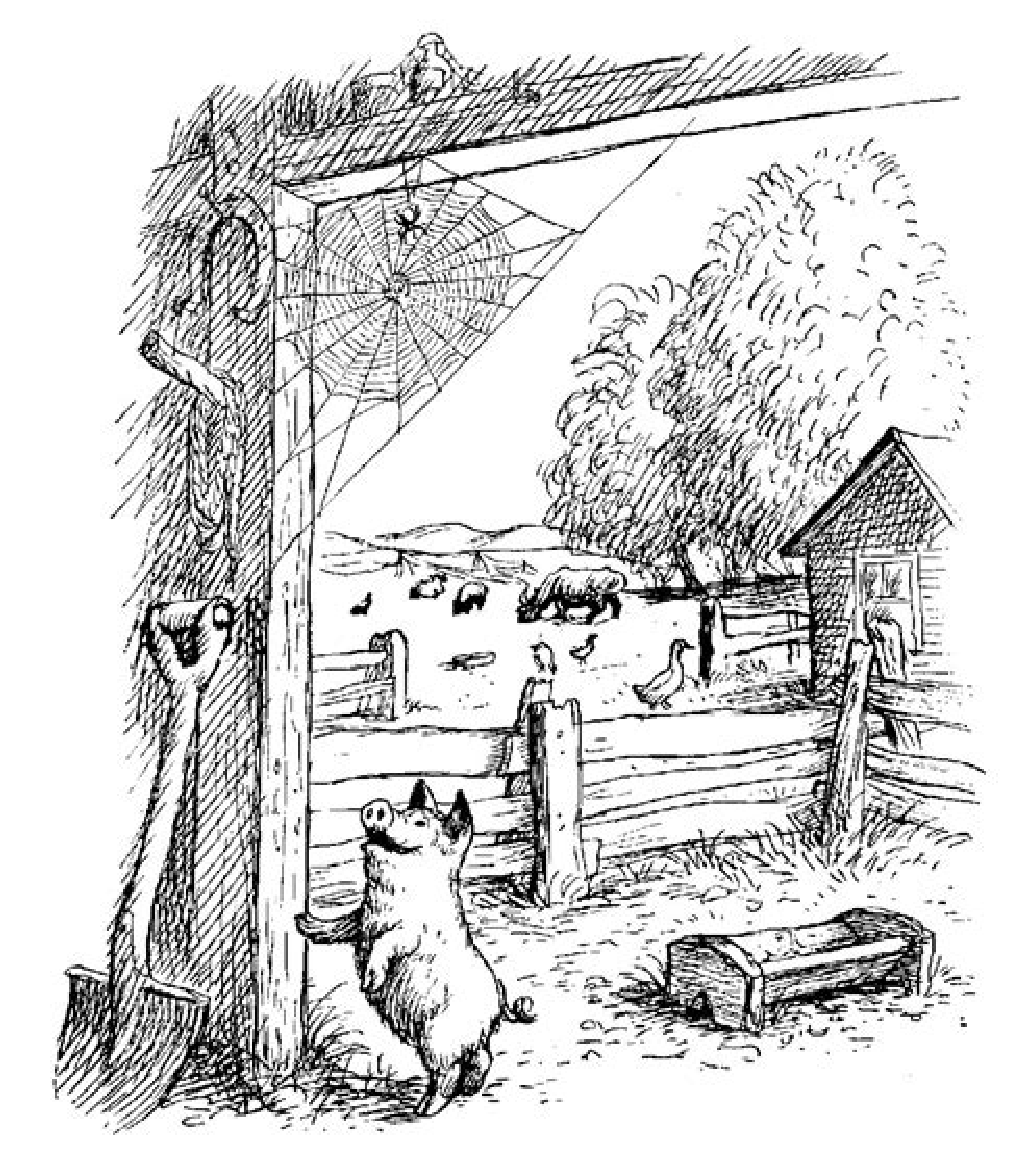
\includegraphics[scale=0.5]{cover.eps} % also works with logo.pdf
    \vfill
		{\noindent Produced by \LaTeXe{}~~\plogo}\\[\baselineskip] % Publisher and logo
	}

  \end{titlepage}


 \tableofcontents


 \chapter{Before Breakfast}

 %%
 
``Where's Papa going with the ax?'' said Fern to her mother as they  \marginpar{ax/axe \tipaencoding{[{\ae}ks]}}
were setting the table for breakfast.                                \index{ax} \index{axe} \index{breakfast}

 ``Out to the hoghouse,'' replied Mrs. Arable. ``Some pigs were born
last night.''                                                        \marginpar{last year, last night}

 ``I don't see why he needs an ax,'' continued Fern, who was only
eight.

 ``Well,'' said her mother, ``one of the pigs is a runt. It's very small 
and weak, and it will never amount to anything. So your father has
decided to do away with it.''                                          \marginpar{runt \tipaencoding{[r2nt]}}

``Do away with it?'' shrieked Fern. ``You mean kill it? Just because  
it's smaller than the others?''

 Mrs. Arable put a pitcher of cream on the table. ``Don't yell,
Fern!'' she said. ``Your father is right. The pig would probably die
anyway.'' 

Fern pushed a chair out of the way and ran outdoors. The grass 
was wet and the earth smelled of springtime. Fern's sneakers were           \index{sneakers}
sopping by the time she caught up with her father.                           \marginpar{is $\rightarrow$ was\\are $\rightarrow$ were}

 ``Please don't kill it!'' she sobbed. ``It's unfair.''                         \index{unfair}
 
Mr. Arable stopped walking.

 ``Fer,'' he said gently, ``you will have to learn to control yourself.''
 
 ``Control myself?'' yelled Fern. ``This is a matter of life and death,
and you talk about controlling myself.'' Tears ran down her cheeks
and she took hold of the ax and tried to pull it out of her father's
hand.

 ``Fern,'' said Mr. Arable, ``I know more about raising a litter of pigs
than you do. A weakling makes trouble. Now run along!''

 ``But it's unfair,'' cried Fern. ``The pig couldn't help being born
small, could it? If I had been very small at birth, would you have
killed me?'' 

Mr. Arable smiled. ``Certainly not,'' he said, looking down at his
daughter with love. ``But this is different. A little girl is one thing, a
little runty pig is another.''

 ``I see no difference,'' replied Fern, still hanging on to the ax. ``This
is the most terrible case of injustice I ever heard of.''
 A queer look came over John Arable's face. He seemed almost
ready to cry himself. 

 ``All right,'' he said.``You go back to the house and I will bring the
runt when I come in. I'll let you start it on a bottle, like a baby.
Then you'll see what trouble a pig can be.''

 When Mr. Arable returned to the house half an hour later, he
carried a carton under his arm. Fern was upstairs changing her                 \marginpar{carton \tipaencoding{["kA:rtn]}\\ \\ cartoon \tipaencoding{[kA:r"tu:n]}}
sneakers. The kitchen table was set for breakfast, and the room
smelled of coffee, bacon, damp plaster, and wood smoke from the
stove. 

 ``Put it on her chair!'' said Mrs. Arable. Mr. Arable set the carton
down at Fern's place. Then he walked to the sink and washed his
hands and dried them on the roller towel.

 Fern came slowly down the stairs. Her eyes were red from crying.
As she approached her chair, the carton wobbled, and there was a
scratching noise... Fern looked at her father. Then she lifted the lid
of the carton. There, inside, looking up at her, was the newborn pig.
It was a white one. The morning light shone through its ears,
turning them pink. 

 ``He's yours,'' said Mr. Arable. ``Saved from an untimely death.
And may the good Lord forgive me for this foolishness.''

 Fern couldn't take her eyes off the tiny pig. ``Oh,'' she whispered.
``Oh, look at him! He's absolutely perfect.'' 

She closed the carton carefully. First she kissed her father, then               \index{carefully}
she kissed her mother. Then she opened the lid again, lifted the pig
out, and held it against her cheek. At this moment her brother
Avery came into the room. Avery was ten. He was heavily
armed---an air rifle in one hand, a wooden dagger in the other. 

``What's that?'' he demanded. ``What's Fern got?''

 ``She's got a guest for breakfast,'' said Mrs. Arable. ``Wash your
hands and face, Avery!''

 ``Let's see it!'' said Avery, setting his gun down. ``You call that
miserable thing a pig? That's a fine specimen of a pig---it's no bigger
than a white rat.''

 ``Wash up and eat your breakfast, Avery!'' said his mother. ``The
school bus will be along in half an hour.''

 ``Can I have a pig, too, Pop?'' asked Avery.
 
 ``No, I only distribute pigs to early risers,'' said Mr. Arable. ``Fern
was up at daylight, trying to rid world of injustice. As a result, she
now has a pig. A small one, to be sure, but nevertheless a pig. It
just shows what can happen if a person gets out of bed promptly.
Let's eat!'' 

But Fern couldn't eat until her pig had had a drink of milk. Mrs.                   \marginpar{not $\cdots$ until}
Arable found a baby's nursing bottle and a rubber nipple. She
poured warm milk into the bottle, fitted the nipple over the top,
and handed it to Fern. ``Give him his breakfast!'' she said. 

A minute later, Fern was seated on the floor in the corner of the
kitchen with her infant between her knees, teaching it to suck from
the bottle. The pig, although tiny, had a good appetite and caught
on quickly. 

The school bus honked from the road.                                  \index{school bus} \index{road}

 ``Run!'' commanded Mrs. Arable, taking the pig from Fern and
slipping a doughnut into her hand. Avery grabbed his gun and
another doughnut.

 The children ran out to the road and climbed into the bus. Fern
took no notice of the others in the bus. She just sat and stared out \marginpar{sit $\rightarrow$ sat}
of the window, thinking what a blissful world it was and how lucky
she was to have entire charge of a pig. By the time the bus reached
school, Fern had named her pet, selecting the most beautiful name
she could think of. 

``Its name is Wilbur,'' she whispered to herself.

 She was still thinking about the pig when the teacher said: `` Fern,
what is the capital of Pennsylvania?''

 ``Wilbur,'' replied Fern, dreamily. The pupils giggled. Fern
blushed.                                                            \marginpar{pupil}

\vspace{2cm}

%%句型练习

\bgroup
\fontfamily{ptm}\selectfont

{\Huge Exercises}

{
\large

 \begin{enumerate}
  \item \textbf{be called$\cdots$}
      \begin{itemize}
          \item This tiny pig was called \textit{Wilbur}, so we can call it \textit{Wilbur}.
          
          \item Hello everyone, I am from China, and I am called \textit{Qucy Yang}. You can call me \textit{Qucy}.
      \end{itemize}
   
   \item \textbf{be smaller than $\cdots$}
      \begin{itemize}
          \item \textit{Wilbur} was smaller than his brothers.
          
          \item But Fern couldn't eat until her pig had had a drink of milk.
      \end{itemize}
   
   \item \textbf{not $\cdots$ until}
      \begin{itemize}
          \item I didn't have dinner until I finished my homework yesterday.
          
          \item Cats are smaller than Tigers.
      \end{itemize}
      
   \item She just sat and stared out of the window, thinking what a blissful world it was and how lucky she was to have entire charge of a pig. 
   
   
 \end{enumerate}
 
}
\egroup



 \chapter{Wilbur}
 
 %%
 
 Fern loved Wilbur more than anything. She loved to stroke him,
to feed him, to put him to bed. Every morning, as soon as she got                \marginpar{as soon as}
up, she warmed his milk, tied his bib on, and held the bottle for
him. Every afternoon, when the school bus stopped in front of her
house, she jumped out and ran to the kitchen to fix another bottle
for him. She fed him again at suppertime, and again just before
going to bed. Mrs. Arable gave him a feeding around noontime
each day, when Fern was away in school. Wilbur loved his milk,
and he was never happier than when Fern was warming up a bottle
for him. He would stand and gaze up at her with adoring eyes. 

For the first few days of his life, Wilbur was allowed to live in a             \marginpar{be allowed to}
box near the stove in the kitchen. Then when Mrs. Arable
complained, he was moved to a bigger box in the woodshed. At two
weeks of age, he was moved outdoors. It was apple-blossom time,
and the days were getting warmer. Mr. Arable fixed a small yard                  \marginpar{is $\rightarrow$ was\\are $\rightarrow$ were}
specially for Wilbur under an apple tree, and gave him a large
wooden box full of straw, with a doorway cut in it so he could walk
in and out as he pleased. 

``Won't he be cold at night?'' asked Fern.

 ``No,'' said her father. ``Your watch and see what he does.'' 

  Carrying a bottle of milk, Fern sat down under the apple tree
inside the yard. Wilbur ran to her and she held the bottle for him 
while he sucked. When he had finished the last drop, he grunted
and walked sleepily into the box. Fern peered through the door. 

Wilbur was poking the straw with his snout. In a short time he had
dug a tunnel in the straw. He crawled into the tunnel and
disappeared from sight, completely covered with straw. Fern was
enchanted. It relieved her mind to know that her baby would sleep
covered up, and would stay warm. 

Every morning after breakfast, Wilbur walked out to the road with
Fern and waited with her till the bus came. She would wave
good-bye to him, and he would stand and watch the bus until it
vanished around a turn. While Fern was in school, Wilbur was shut
up inside his yard. But as soon as she got home in the afternoon,
she would take him out and he would follow her around the place. 

If she went into the house, Wilbur went, too. If she went upstairs,
Wilbur would wait at the bottom step until she came down again. If
she took her doll for a walk in the doll carriage, Wilbur followed
along. Sometimes, on these journeys, Wilbur would get tired, and             \marginpar{get tired}
Fern would pick him up and put him in the carriage alongside the
doll. He liked this. And if he was very tired, he would close his eyes
and go to sleep under the doll's blanket. He looked cute when his 
eyes were closed, because his lashes were so long. The doll would 
close her eyes, too, and Fern would wheel the carriage very slowly
and smoothly so as not to wake her infants. 

One warm afternoon, Fern and Avery put on bathing suits and
went down to the brook for a swim. Wilbur tagged along at Fern's
heels. When she waded into the brook, Wilbur waded in with her.
He found the water quite cold--too cold for his liking. So while the
children swam and played and splashed water at each other,
Wilbur amused himself in the mud along the edge of the brook,
where it was warm and moist and delightfully sticky and oozy. 

Every day was a happy day, and every night was peaceful.

 Wilbur was what farmers call a spring pig, which simply means
that he was born in springtime. When he was five weeks old, Mr.
Arable said he was now big enough to sell, and would have to be
sold. Fern broke down and wept. But her father was firm about it.
Wilbur's appetite had increased; he was beginning to eat scraps of
food in addition to milk. Mr. Arable was not willing to provide for
him any longer. He had already sold Wilbur's ten brothers and
sisters. 

``He's got to go, Fern,'' he said. ``You have had your fun raising a
baby pig, but Wilbur is not a baby any longer and he has got to be
sold.'' 

 ``Call up the Zuckermans,'' suggested Mrs. Arable to Fern. ``Your 
Uncle Homer sometimes raises a pig. And if Wilbur goes there to
live, you can walk down the road and visit him as often as you like.'' 

``How much money should I ask for him?'' Fern wanted to know.

 ``Well,'' said her father, ``he's a runt. Tell your Uncle Homer you've
got a pig you'll sell for six dollars, and see what he says.''

 It was soon arranged. Fern phoned and got her Aunt Edith, and
her Aunt Edith hollered for Uncle Homer, and Uncle Homer came
in from the barn and talked to Fern. When he heard that the price
was only six dollars, he said he would buy the pig. Next day Wilbur
was taken from his home under the apple tree and went to live in a
manure pile in the cellar of Zuchkerman's barn. 

%%句型练习
\vspace{1cm}

\bgroup
\fontfamily{ptm}\selectfont

{\Huge Exercises}

{
\large

 \begin{enumerate}
  \item \textbf{as soon as}
      \begin{itemize}
          \item As soon as we opened the front door we could smell the gas.
          
          \item Wilbur, finish your homework as soon as possible!
      \end{itemize}
   
  
 \end{enumerate}
 
}
\egroup


 \chapter{Escape}
 
 The barn was very large. It was very old. It smelled of hay and it
smelled of manure. It smelled of the perspiration of tired horses
and the wonderful sweet breath of patient cows. It often had a sort
of peaceful smell -- as though nothing bad could happen ever again
in the world. It smelled of grain and of harness dressing and of axle
grease and of rubber boots and of new rope. And whenever the cat 
was given a fish-head to eat, the barn would smell of fish. But
mostly it smelled of hay, for there was always hay in the great loft
up overhead. And there was always hay being pitched down to the
cows and the hourses and the sheep.

The barn was pleasantly warm in winter when the animals spent
most of their time indoors, and it was pleasantly cool in summer  \marginpar{pleasantly}
when the big doors stood wide open to the breeze. The barn had
stalls on the main floor for the work hourses, tie-ups on the main
floor for the cows, a sheepfold down below for the sheep, a pigpen
down below for Wilbur, and it was full of all sorts of things that you
find in barns: ladders, grindsones, pitch forks, monkey wrenches,
scythes, lawn mowers, snow shovels, ax handles, milk pails, water
buchers, empty grain sacks, and rusty rat traps. It was the kind of
barn that swallows like to build their nests in. It was the kind of
barn that children like to play in. And the whole thing was owned
by Fern's uncle, Mr. Homer L. Zuckerman. 

Wilbur's new home was in the lower part of the barn, directly
underneath the cows. Mr. Zuckerman knew that a manure pile is a  \marginpar{underneath}
good place to keep a young pig. Pigs need warmth, and it was
warm and comfortable down there in the barn cellar on the south
side. 

Fern came almost every day to visit him. She found an old milking
stool that had been discarded, and she placed the stool in the
sheepfold next to Wilbur's pen. Here she sat quietly during the
long afternoos, thinking and listening and watching Wilbur. The
sheep soon got to know her and trust her. So did the geese, who
lived with the sheep. All the animals trusted her, she was so quiet
and friendly. Mr. Zuckerman did not allow her to take Wilbur out,
and he did not allow to git into the pigpen. But he told Fern that
she could sit on the stool and watch Wilbur as long as she wanted
to. It made her happy just to be near the pig, and it made her
happy just to be near the pig, and it made Wilbur happy to know
that she was sitting there, right outside his pen. But he never had
any fun--no walks, no redes, no swims. 

One afternoon in June, when Wilbur was almost two months old,
he wandered out into his smalll yard outside the barn. Fern had
not arrived for her usual visit. Wilbur stood in the sun feeling
lonely and bored.

 ``There's never anything to do around here,'' he thought. He
walked slowly to his food trough and sniffed to see if anything had  \marginpar{sniff}
been overlooked at lunch. He found a small strip of potato skin and
ate it. His back itched, so he leaned against the fence and rubbed
against the boards. When he tired of this, he walked indoors, 
climbed to the top of the manured pile , and sat down. He didn't
feel like going to sleep, he didn't feel like digging, he was tired of
standing still, tired of lying down. ``I'm less than two months old
and I'm tired of living,'' he said. He walked out to the yard again.

 ``When I'm out here,'' he said, ``there's no place to go but in. When
I'm indoors, there's no place to go but out in the yard.'' 
 
 ``That's where you're wrong, my friend, my freiend,'' said a voice.
 
 Wilbur looked through the fence and saw the goose standing there.
 
 ``You don't have to stay in that dirty-llittle dirty-little dirty-little
yard,'' said the goose, who talded rather fast. ``One of the boards is
loose. Push on it, push-push-push on it, and come on out!''                            \marginpar{loose \tipaencoding{[lu:s]}}

 ``What?'' said Wilbur. ``Say it slower!''
 
  ``At-at-at, at the risk of repeating myself,'' said the goose, ``I
suggest that you come on out. It's wonderful out here.''

 ``Did you say a board was loose?''
 
 ``That I did, that I did,'' said the goose.
 
 Wilbur walked up to the fence and saw that the goose was
right--one board was loose. He put his head sown, shut his eyes,
and pushed. The board gave way. In a minute he had squeezed
through the fence and was standing in the long grass outside his
yard. The goose chuckled. 
 
``How does it feel to be free?'' she asked.

 ``I like it ,'' said Wilbur. ``That is, I guess Ilike it.'' Actually, Wilbur
felt queer to be out side his fence, with nothing between him and
the big world.

 ``Where do you think I'd better go?''  
 
  ``Anywhere you like, anywhere you like,'' said the goose. ``Go down
through the orchard, root up the sod! Go down through the garden,
dig up the radishes! Root up everything! Eat grass! Look for corn!
Look for oats! Run all over! Skip and dance, jump and prance! Go
down through the orchard and stroll in the woods! The world is a
wonderful place when you're young.'' 
  
``I can see that,'' replied Wilbur. He gave a jump in the air, twirled,
ran a few steps, stopped, looked all around, sniffed the smells of
afternoon, and then set off walking down through the orchard.
Pausing in the shade of an apple tree, he put his strong snout into
the ground and began pushing, digging, and rooting. He felt very
happy. He had plowed up quite a piece of ground before anyone
noticed him. Mrs. Zuckerman was the first to see him. She saw him
from the kitchen window, and she immediately shouted for the 
men. 

``Ho-mer!'' she cried. ``Pig's out! Lurvy! Pig's out! Homer! Lurvy!
Pig's out. He's down there under that apple tree.''

 ``Now the trouble starts,'' thought Wilbur.`` Now I'll catch it.''
 
 The goose heard the racket and she, too, started hollering.
``Run-run-run downhill, make for the woods, the woods!'' she
shouted to Wilbur. ``They'll never-never-never catch you in the
woods.'' 
  
The cocker spaniel heard the commotion and he ran out from the
barn to join the chase. Mr. Zuckerman heard, and he came out of
the machine shed where he was mending a tool. Lurvy, the hired
man, heard the noise and came up from the asparagus patch where
he was pulling weeds. Everybody walked toward Wilbur and
Wilbur didn't know what to do. The woods seemed a long way off,
and anyway, he had never been down there in the woods and
wasn't sure he would like it.

 ``Get around behind him, Lurvy,'' said Mr. Zuckerman, ``and drive
him toward the barn! And take it easy-don't rush him! I'll go and
get a bucket of slops.''   
  
The news of Wilbur's escape spread rapidly among the animals on
the place. Whenever any creature broke loose on Zuckerman's farm, 
the event was of great interest to the others. The goose shouted to
the nearest cow that Wilbur was free, and soon all the cows knew.
Then one of the cows told one of the sheep, and soon all the sheep
knew. The lambs learned about it from their mothers. The horses,
in their stalls in the barn, pricked up their ears when they heard
the goose hollering; and soon the horses had caught on to what was
happening. ``Wilbur's out,'' they said. Every animal stirred and
lifted its head and became excited to know that one of his friends
had got free and was no longer penned up or tied fast. 

Wilbur didn't know what to do or which way to run. It seemed as
through everybody was after him.`` If this is what it's like to be
free,'' he thought,`` I believe I'd rather be penned up in my own
yard.''

 The cocker spaniel was sneaking up on him from one side. Lurvy
the hired man was sneaking up on him from the other side. Mrs.
Zuckerman stood ready to head him off if he started for the garden,
and now Mr. Zuckerman was coming down toward him carrying a
pail.`` This is really awful,'' thought Wilbur. ``Why doesn't Fern
come?'' He began to cry. 
  
The goose took command and began to give orders. 

 ``Don't just stand there, Wilbur! Dodge about, dodge about!'' cried
the goose.`` Skip around, run toward me, slip in and out, in and out,
in and out! Make for the woods! Twist and turn!''

 The cocker spaniel sprang for Wilbur's hind leg. Wilbur jumped
and ran. Lurvy reached out and grabbed. Mrs. Zuckerman
screamed at Lurvy. The goose cheered for Wilbur. Wilbur dodged
between Lurvy's legs. Lurvy missed Wilbur and grabbed the
spaniel instead. ``Nicely done, nicely done!'' cried the goose.`` Try it
again, try it again!'' 

 ``Run downhill!'' suggested the cows.
 
 ``Run toward me!'' yelled the gander.
 
 ``Run uphill!'' cried the sheep.
 
 ``Turn and twist!'' honked the goose.
 
 ``Jump and dance!'' said the rooster.
 
 ``Look out for Lurvy!'' called the cows.
 
 ``Look out for Zuckerman!'' yelled the gander.
 
 ``Watch out for the dog!'' cried the sheep.
 
 ``Listen to me, listen to me!'' screamed the goose. 
 
 Poor Wilbur was dazed and frightened by this hullabaloo. He
didn't like being the center of all this fuss. He tried to follow the
instructions his friends were giving him, but he couldn't run
downhill and uphill at the same time, and he couldn't turn and 
twist when he was jumping and dancing, and he was crying so hard
he could barely see anything that was happening. After all, Wilbur
was a very young pig-not much more than a baby, really. He
wished Fern were there to take him in his arms and comfort him.

When he looked up and saw Mr. Zuckerman standing quite close to
him, holding a pail of warm slops, he felt relieved. He lifted his
nose and sniffed. The smell was delicious-warm milk, potato skins,
wheat middlings, Kellogg's Corn Flakes, and a popover left from
the Zuckermans' breakfast. 
 
 ``Come, pig!'' said Mr. Zuckerman, tapping the pail. ``Come pig!''
 Wilbur took a step toward the pail.
 
 ``No-no-no!'' said the goose. ``It's the old pail trick, Wilbur. Don't
fall for it, don't fall for it ! He's trying to lure you back into
captivity-ivity. He's appealing to your stomach.''

 Wilbur didn't care. The food smelled appetizing. He took another
step toward the pail.

 ``Pig, pig!'' said Mr. Zuckerman in a kind voice, and began walking
slowly toward the barnyard, looking all about him innocently, as if
he didn't know that a little white pig was following along behind
him.

 ``You'll be sorry-sorry-sorry,'' called the goose. 
 
Wilbur didn't care. He kept walking toward the pail of slops. 

 ``You'll miss your freedom,'' honked the goose. ``An hour of
freedom is worth a barrel of slops.''

 Wilbur didn't care.
 
 When Mr. Zuckerman reached the pigpen, he climbed over the
fence and poured the slops into the trough. Then he pulled the
loose board away from the fence, so that there was a wide hole for
Wilbur to walk through.

 ``Reconsider, reconsider!'' cried the goose.  

  Wilbur paid no attention. He stepped through the fence into his
yard. He walked to the trough and took a long drink of slops,
sucking in the milk hungrily and chewing the popover. It was good
to be home again.

 While Wilbur ate, Lurvy fetched a hammer and some 8-penny
nails and nailed the board in place. Then he and Mr. Zuckerman
leaned lazily on the fence and Mr. Zuckerman scratched Wilbur's
back with a stick.

 ``He's quite a pig,'' said Lurvy.
 
 ``Yes, he'll make a good pig,'' said Mr. Zuckerman.
 
 Wilbur heard the words of praise. He felt the warm milk inside his
stomach. He felt the pleasant rubbing of the stick along his itchy
back. He felt peaceful and happy and sleepy. This had been a tiring
afternoon. It was still only about four o'clock but Wilbur was ready 
for bed.

 ``I'm really too young to go out into the world alone,'' he thought
as he lay down.


 
  \chapter{Loneliness}
 
 The next day was rainy and dark. Rain fell on the roof of the barn
and dripped steadily from the eaves. Rain fell in the barnyard and
ran in crooked courses down into the lane where thistles and
pigweed grew. Rain spattered against Mrs. Zuckerman's kitchen
windows and came gushing out of the downspouts. Rain fell on the
backs of the sheep as they grazed in the meadow. When the sheep
tired of standing in the rain, they walked slowly up the lane and
into the fold.

 Rain upset Wilbur's plans. Wilbur had planned to go out, this day,
and dig a new hole in his yard. He had other plans, too. His plans
for the day went something like this: 

Breakfast at six-thirty. Skim milk, crusts, middlings, bits of
doughnuts, wheat cakes with drops of maple syrup sticking to them,
potato skins, leftover custard pudding with raisins, and bits of 
Shredded Wheat.

 Breakfast would be finished at seven.
 
 From seven to eight, Wilbur planned to have a talk with
Templeton, the rat that lived under his trough. Talking with
Templeton was not the most interesting occupation in the world
but it was better than nothing.

 From eight to nine, Wilbur planned to take a nap outdoors in the
sun. 

From nine to eleven he planned to dig a hole, or trench, and
possibly find something good to eat buried in the dirt.

 From eleven to twelve he planned to stand still and watch flies on
the boards, watch bees in the clover, and watch swallows in the air.

 Twelve o'clock-lunchtime. Middlings, warm water, apple parings,
meat gravy, carrot scrapings, meat scraps, stale hominy, and the
wrapper off a package of cheese. Lunch would be over at one.

 From one to two, Wilbur planned to sleep.
 
 From two to three, he planned to scratch itchy places by rubbing
against the fence.

 From three to four, he planned to stand perfectly still and think of
what it was like to be alive, and to wait for Fern. 

 At four would come supper. Skim milk, provender, leftover
sandwich from Lurvy's lunchbox, prune skins, a morsel of this, a 
bit of that, fried potatoes, marmalade drippings, a little more of
this, a little more of that, a piece of baked apple, a scrap of upside
down cake.

 Wilbur had gone to sleep thinking about these plans. He awoke at
six and saw the rain, and it seemed as though he couldn't bear it.

 ``I get every thing all beautifully planned out and it has to go and
rain,'' he said.

 For a while he stood gloomily indoors. Then he walked to the door
and looked out. Drops of rain struck his face. His yard was cold
and wet. his trough had and inch of rainwater in it. Templeton was
nowhere to be seen. 

``Are you out there, Templeton?'' called Wilbur. There was no
answer. Suddenly Wilbur felt lonely and friendless.

 ``One day just like another,'' he groaned. ``I'm very young, I have
no real friend here in the barn, it's going to rain all morning and all
afternoon, and Fern won't come in such bad weather. Oh,
honestly!'' And Wilbur was crying again, for the second time in two
days.

 At six-thirty Wilbur heard the banging of a pail. Lurvy was
standing outside in the rain, stirring up breakfast.

 ``C'mon, pig!'' said Lurvy.
 
 Wilbur did not budge. Lurvy dumped the slops, scraped the pail 
and walked away. He noticed that something was wrong with the
pig. 

 Wilbur didn't want food, he wanted love. He wanted a
friend--someone who would play with him. He mentioned this to
the goose, who was sitting quietly in a corner of the sheepfold.

 ``Will you come over and play with me?'' he asked.
 
 ``Sorry, sonny, sorry,'' said the goose. ``I'm sitting-sitting on my
eggs. Eight of them. Got to keep them toasty-oasty-oasty warm. I
have to stay right here, I'm no flibberty-ibberty-gibbet. I do not
play when there are eggs to hatch. I'm expecting goslings.''

 ``Well, I didn't think you were expecting wood-peckers,'' said
Wilbur, bitterly.

 Wilbur next tried one of the lambs.
 
 ``Will you please play with me?'' he asked.
 
 ``Certainly not,'' said the lamb. ``In the first place, I cannot get into
your pen, as I am not old enough to jump over the fence. In the
second place, I am not interested in pigs. Pigs mean less than
nothing to me.'' 

 ``What do you mean, less than nothing?'' replied Wilbur. ``I don't
think there is any such thing as less than nothing. Nothing is
absolutely the limit of nothingness. It's the lowest you can go. It's
the end of the line. How can something be less than nothing? If 
there were something that was less than nothing, then nothing
would not be nothing, it would be something--even though it's just
a very little bit of something. But if nothing is nothing, then
nothing has nothing that is less than it is.''

 ``Oh, be quiet!'' said the lamb. ``Go play by yourself! I don't play
with pigs.''

Sadly, Wilbur lay down and listened to the rain. Soon he saw the
rat climbing down a slanting board that he used as a stairway.

 ``Will you play with me, Templeton?'' asked Wilbur.
 
 ``Play?'' said Templeton, twirling his whiskers. ``Play? I hardly
know the meaning of the word.''

 ``Well,'' said Wilbur, ``it means to have fun, to frolic, to run and
skip and make merry.'' 

 ``I never do those things if I can avoid them, '' replied the rat,
sourly. ``I prefer to spend my time eating, gnawing, spying, and
hiding. I am a glutton but not a merry-maker. Right now I am on
my way to your trough to eat your breakfast, since you haven't got
sense enough to eat it yourself.'' And Templeton, the rat, crept
stealthily along the wall and disappeared into a private tunnel that
he had dug between the door and the trough in Wilbur's yard.

Templeton was a crafty rat, and he had things pretty much his own 
way. The tunnel was an example of his skill and cunning. The
tunnel enabled him to get from the barn to his hiding place under
the pig trough without coming out into the open. He had tunnels
and runways all over Mr. Zuckerman's farm and could get from
one place to another without being seen. Usually he slept during
the daytime and was abroad only after dark. 

 Wilbur watched him disappear into his tunnel. In a moment he
saw the rat's sharp nose poke out from underneath the wooden
trough. Cautiously Templeton pulled himself up over the edge of
the trough. This was almost more than Wilbur could stand: on this
dreary, rainy day to see his breakfast being eaten by somebody else.
He knew Templeton was getting soaked, out there in the pouring
rain, but even that didn't comfort him. Friendless, dejected, and
hungry, he threw himself down in the manure and sobbed.

 Late that afternoon, Lurvy went to Mr. Zuckerman. ``I think
there's something wrong with that pig of yours. He hasn't touched
his food.''

 ``Give him two spoonfuls of sulphur and a little molasses,'' said Mr.
Zuckerman. 

 Wilbur couldn't believe what happening to him when Lurvy
caught him and forced the medicine down his throat. This was
certainly the worst day of his life. He didn't know whether he could 
endure the awful loneliness any more.

 Darkness settled over everything. Soon there were only shadows
and the noises of the sheep chewing their cuds, and occasionally
the rattle of a cow-chain up overhead. You can imagine Wilbur's
surprise when, out of the darkness, came a small voice he had
never heard before. It sounded rather thin, but pleasant. ``Do you
want a friend, Wilbur?'' it said. ``I'll be a friend to you. I've watched
you all day and I like you.''

 ``But I can't see you,'' said Wilbur, jumping to his feet. ``Where are
you? And who are you?'' 

 ``I'm right up here,'' said the voice. ``Go to sleep. You'll see me in
the morning.'' 


 
   \chapter{Charlotte}

The night seemed long. Wilbur's stomach was empty and his
mind was full. And when your stomach is empty and your mind is
full, it's always hard to sleep.

 A dozen times during the night Wilbur woke and stared into the
blackness, listening to the sounds and trying to figure out what
time it was. A barn is never perfectly quiet. Even at midnight there 
is usually something stirring. 

 The first time he woke, he heard Templeton gnawing a hole in the
grain bin. Templeton's teeth scraped loudly against the wood and
made quite a racket. ``That crazy rat!'' thought Wilbur. ``Why does
he have to stay up all night, grinding his clashers and destroying
people's property? Why can't he go to sleep, like any decent
animal?''

 The second time Wilbur woke, he heard the goose turning on her
nest and chuckling to herself.

 ``What time is it?'' whispered Wilbur to the goose.
 
 ``Probably-obably-obably about half-past eleven,'' said the goose,
``Why aren't you asleep, Wilbur?''

 ``Too many things on my mind,'' said Wilbur.
 
 ``Well,'' said the goose, ``that's not my trouble. I have nothing at all
on my mind, but I've too many things under my behind. Have you
ever tried to sleep while sitting on eight eggs?''

 ``No,'' replied Wilbur, ``I suppose it is uncomfortable. How long
does it take a goose egg to hatch?'' 

 ``Approximately-oximately thirty days, all told,'' answered the
goose. ``But I cheat a little. On warm afternoons, I just pull a little
straw over the eggs and go out for a walk.''

 Wilbur yawned and went back to sleep. In his dreams he heard 
again the voice saying, ``I'll be a friend to you. Go to sleep--you'll
see me in the morning.'' 

 About half an hour before dawn, Wilbur woke and listened. The
barn was still dark. The sheep lay motionless. Even the goose was
quiet. Overhead, on the main floor, nothing stirred: the cows were
resting, the horses dozed. Templeton had quit work and gone off
somewhere on an errand. The only sound was a slight scraping
noise from the rooftop, where the weather-vane swung back and
forth. Wilbur loved the barn when it was like this--calm and quiet,
waiting for light.

 ``Day is almost here,'' he thought.
 
 Through a small window, a faint gleam appeared.
 
One by one the stars went out. Wilbur could see the goose a few
feet away. She sat with head tucked under a wing. Then he could
see the sheep and the lambs. The sky lightened.

 ``Oh, beautiful day, it is here at last! Today I shall find my friend.'' 
 
Wilbur looked everywhere. He searched his pen thoroughly. He
examined the window ledge, stared up at the ceiling. But he saw
nothing new. Finally he decided he would have to speak up. He
hated to break the lovely stillness of dawn by using his voice, but
he couldn't think of any other way to locate the mysterious new
friend who was nowhere to be seen. So Wilbur cleared his throat. 

 ``Attention, please!'' he said in a loud, firm voice. ``Will the party
who addressed me at bedtime last night kindly make himself or
herself known by giving an appropriate sign or signal!''

 Wilbur paused and listened. All the other animals lifted their
heads and stared at him. Wilbur blushed. But he was determined
to get in touch with his unknown friend. 

``Attention, please!'' he said. ``I will repeat the message. Will the
party who addressed me at bedtime last night kindly speak up.
Please tell me where you are, if you are my friend!''

 The sheep looked at each other in disgust.

 ``Stop your nonsense, Wilbur!'' said the oldest sheep. ``If you have
a new freind here, you are probably disturbing his rest; and the
quickest way to spoil a friendship is to wake somebody up in the
morning before he is ready. How can you be sure your friend is an
early riser?''

 ``I beg everyone's pardon,'' whispered Wilbur. ``I didn't mean to be
objectionable.''

 He lay down meekly in the in the manure, facing the door. He did
not know it, but his friend was very near. and the old sheep was
right--the friend was still asleep. 

 Soon Lurvy appeared with slops for breakfast. Wilbur rushed out,
ate everything in a hurry, and licked the trough. The sheep moved 
off down the lane, the gander waddled along behind them, pulling
grass. And then, just as Wilbur was settling down for his morning
nap, he heard again the thin voice that had addressed him the
night before.

 ``Salutations!'' said the voice.

 Wilbur jumped to his feet. ``Salu-what?'' he cried.

 ``Salutations!'' said the voice.

 ``What are they, and where are you?'' screamed Wilbur. ``Please,
please, tell me where you are. And what are salutations?''

``Salutations are greetings,'' said the voice. ``When I say
'salutations,' it's just my fancy way of saying hello or good morning.
Actually, it's a silly expression, and I am surprised that I used it at
all. As for my whereabouts, that's easy. Look up here in the corner
of the dooway! Here I am. Look, I'm waving!''

 At last Wilbur saw the creature that had spoken to him in such a
kindly way. Stretched across the upper part of the doorway was a
big spiderweb, and hanging from the top of the web, head down,
was a large grey spider. She was about the size of a gumdrop. She
had eight legs, and she was waving one of them at Wilbur in
friendly greeting. ``See me now?'' she asked. 

``Oh, yes indeed,'' said Wilbur. ``Yes indeed! How are you? Good
morning! Salutations! Very pleased to meet you. What is your
name, please? May I have your name?''

 ``My name,'' said the spider,`` is Charlotte.''

 ``Charlotte what?'' asked Wilbur, eagerly.

 ``Charlotte A. Cavatica. But just call me Charlotte.''

 ``I think you're beautiful,'' said Wilbur.

 ``Well, I am pretty,'' replied Charlotte. ``There's no denying that.
Almost all spiders are rather nice-looking. I'm not as flashy as
some, but I'll do. I wish I could see you, Wilbur, as clearly as you
can see me.''

 ``Yes, but I'm near-sighted,'' replied Charlotte. ``I've always
been dreadfully near-sighted. It's good in some ways, not so good
in others. Watch me wrap up this fly.''

``Why can't you?'' asked the pig. ``I'm right here.'' 

  A fly that had been crawling along Wilbur's trough had flown up
and blundered into the lower part of Charlotte's web and was
tangled in the sticky threads. The fly was beating its wings
furiously, trying to break loose and free itself. 

 ``First,'' said Charlotte, `` I dive at him.'' She plunged headfirst
toward the fly. As she dropped, a tiny silken thread unwound from
her rear end.

 ``Next, I wrap him up.'' She grabbed the fly, threw a few jets of silk
around it, and rolled it over and over, wrapping it so that it
couldn't move. Wilbur watched in horror. He could hardly believe
what he was seeing, and although he detested flies, he was sorry for
this one.

 ``There!'' said Charlotte. ``Now I knock him out, so he'll be more
comfortable.'' She bit the fly. ``He can't feel a thing now,'' she
remarked. ``He'll make a perfect breakfast for me.''

 ``You mean you eat flies?'' gasped Wilbur.

 ``Certainly. Flies, bugs, grasshoppers, choice beetles, moths,
butterflies, tasty cockroaches, gnats, midges, daddy longlegs,
centipedes, mosquitoes, crickets--anything that is careless enough
to get caught in my web. I have to live, don't I?''

``Why, yes, of course,'' said Wilbur. ``Do they taste good?''

 ``Delicious. Of course, I don't really eat them. I drink them--drink
their blood. I love blood,'' said Charlotte, and her pleasant, thin
voice grew even thinner and more pleasant.

 ``Don't say that!'' groaned Wilbur. ``Please don't say things like
that!'' 

 ``Why not ? It's true, and I have to say what is true. I am not
entirely happy about my diet of flies and bugs, but it's the way I'm
made. A spider has to pick up a living somehow or other, and I
happen to be a trapper. I just naturally build a web and trap flies
and other insects. My mother was a trapper before me. Her mother
was a trapper before her. All our family have been trappers. Way
back for thousands and thousands of years we spiders have been
laying for flies and bugs.''

 ``It's a miserable inheritance,'' said Wilbur, gloomily. He was sad
because his new friend was so bloodthirsty. 

 ``Yes, it is,'' agreed charlotte. ``But I can't help it. I don't know how
the first spider in the early days of the world happened to think up
this fancy idea of spinning a web, but she did, and it was clever of
her, too. And since then, all of us spiders have had to work the
same trick. It's not a bad pitch, on the whole.''

 ``It's cruel,'' replied Wilbur, who did not intend to be argued out of
his position.

 ``Well, you can't talk,'' said Charlotte. ``You have your meals
brought to you in a pail. Nobody feeds me. I have to get my own
living. I live by my wits. I have to be sharp and clever, lest I go
hungry. I have to think things out, catch what I can, take what
comes. Ant it just so happens, my friend, that what comes is flies 
and insects and bugs. And furthermore,'' said Charlotte, shaking
one of her legs, ``do you realize that if I didn't catch bugs and eat
them, bugs would increase and multiply and get so numerous that
they'd destroy the earth, wipe out everything?'' 

 ``Really?'' said Wilbur. ``I wouldn't want that to happen. Perhaps
your web is a good thing after all.''

 The goose had been listening to this conversation and chuckling
to herself. ``There are a lot of things Wilbur doesn't know about
life,'' she thought. ``He's really a very innocent little pig. He doesn't
even know what's going to happen to him around Christmastime;
he has no idea that Mr. Zuckerman and Lurvy are plotting to kill
him.'' And the goose raised herself a bit and poked her eggs a little
further under her so that they would receive the full heat from her
warm body and soft feathers.

 Charlotte stood quietly over the fly, preparing to eat it. Wilbur lay
down and closed his eyes. He was tired from his wakeful night and
from the excitement of meeting someone for the first time. A
breeze brought him the smell of clover--the sweet-smelling world
beyond his fence. ``Well,'' he thought,`` I've got a new friend, all
right. But what a gamble friendship is! Charlotte is fierce, brutal,
scheming, bloodthirsty--everything I don't like. How can I learn to
like her, even though she is pretty and, of course, clever?''

 Wilbur was merely suffering the doubts and fears that often go
with finding a new friend. In good time he was to discover that he
was mistaken about Charlotte. Underneath her rather bold and
cruel exterior, she had a kind heart, and she was to prove loyal and
true to the very end. 

  \chapter{Summer Days}
 The early summer days on a farm are the happiest and fairest
days of the year. Lilacs bloom and make the air sweet, and then
fade. Apple blossoms come with the lilacs, and the bees visit
around among the apple trees. The days grow warm and soft.

School ends, and children have time to play and to fish for trouts in
the brook. Avery often brought a trout home in his pocket, warm
and stiff and ready to be fried for supper.

 Now that school was over, Fern visited the barn almost every day,
to sit quietly on her stool. The animals treated her as an equal. The
sheep lay calmly at her feet. 

 Around the first of July, the work horses were hitched to the
mowing machine, and Mr. Zuckerman climbed into the seat and 
drove into the field. All morning you could hear the rattle of the
machine as it went round and round, while the tall grass fell down
behind the cutter bar in long green swathes. Next day, if there was
no thunder shower, all hands would help rake and pitch and load,
and the hay would be hauled to barn in the high hay wagon, with
Fern and Avery riding at the top of the load. Then the hay would be
hoisted, sweet and warm, into the big loft, until the whole barn
seemed like a wonderful bed of timothy and clover. It was fine to
jump in, and perfect to hide in. And sometimes Avery would find a
little grass snake in the hay, and would add it to the other things in
his pocket. 

 Early summer days are a jubilee time for birds. In the fields,
around the house, in the barn, in the woods, in the
swamp--everywhere love and songs and nests and eggs. From the
edge of the woods, the white-throated sparrow(which must come
all the way from Boston) calls, ``Oh, Peabody, Peabody, Peabody!''
On an apple bough, the phoebe teeters and wags its tail and says,

``Phoebe, phoe-bee!'' The song sparrow, who knows how brief and
lovely life is, says, ``Sweet, sweet, sweet interlude; sweet, sweet,
sweet interlude.'' If you enter the barn, the swallows swoop down
from their nests and scold. ``Cheeky, cheeky!'' they say.

 In early summer there are plenty of things for a child to eat and       
drink and suck and chew. Dandelion stems are full of milk, clover
heads are loaded with nectar, the Frigidaire is full of ice-cold
drinks. Everywhere you look is life; even the little ball of spit on the
weed stalk, if you poke it apart, has a green worm inside it. And on
the under side of the leaf of the potato vine are the bright orange
eggs of the potato bug. 

 It was on a day in early summer that the goose eggs hatched. This
was an important event in the barn cellar. Fern was there, sitting
on her stool, when it happened.

 Except for the goose herself, Charlotte was the first to know that
the goslings had at last arrived. The goose knew a day in advance
that they were coming--she could hear their weak voices calling
from inside the egg. She knew that they were coming. She knew
that they were in a desperately cramped position inside the shell
and were most anxious to break through and get out. So she sat
quite still, and talked less than usual.

 When the first gosling poked its grey-green head through the
goose's feathers and looked around, Charlotte spied it and made
the announcement.

 ``I am sure,'' she said,`` that every one of us here will be gratified to
learn that after four weeks of unremitting effort and patience on
the part of our friend the goose, she now has something to show for 
it. The goslings have arrived. May I offer my sincere
congratulations!'' 

``Thank you, thank you, thank you!'' said the goose, nodding and
bowing shamelessly.

 ``Thank you,'' said the gander.

 ``Congratulations!'' shouted Wilbur. ``How many goslings are
there? I can only see one.''

 ``There are seven,'' said the goose.

 ``Fine!'' said Charlotte. ``Seven is a lucky number.''

 ``Luck had nothing to do with this,'' said the goose. ``It was good
management and hard work.''

 At this point, Templeton showed his nose from his hiding place
under Wilbur's trough. He glanced at Fern, then crept cautiously
toward the goose, keeping close to the wall. Everyone watched him,
for he was not well liked, not trusted.

 ``Look,'' he began in his sharp voice, ``you say you have seven
goslings. There were eight eggs. What happened to the other egg?
Why didn't it hatch?''

 ``It's a dud, I guess,'' said the goose.

 ``What are you going to do with it?'' continued Templeton, his
little round beady eyes fixed on the goose. 

 ``You can have it,'' replied the goose. ``Roll it away and add it to 
that nasty collection of yours.'' (Templeton had a habit of picking
up unusual objects around the farm and storing them in his home.
He saved everything.)

 ``Certainly-ertainly-ertainly,'' said the gander. ``You may have the
egg. But I'll tell you one thing, Templeton, if I ever catch you
poking-oking-oking your ugly nose around our goslings, I'll give
you the worst pounding a rat ever took.'' And the gander opened
his strong wings and beat the air with them to show his power. He
was strong and brave, but the truth is, both the goose and the
gander were worried about Templeton. And with good reason. The
rat had no morals, no conscience, no scruples, no consideration, no
decency, no milk of rodent kindness, no compunctions, no higher
feeling, no friendliness, no anything. He would kill a gosling if he
could get away with it--the goose knew that. Everybody knew it. 

 With her broad bill the goose pushed the unhatched egg out of the
nest, and the entire company watched in disgust while the rat
rolled it away. Even Wilbur, who could eat almost anything, was
appalled. ``Imagine wanting a junky old rotten egg!'' he muttered.

 ``A rat is a rat,'' said Charlotte. She laughed a tinkling little laugh.
``But, my friends, if that ancient egg ever breaks, this barn will be
untenable.'' 

 ``What's that mean?'' asked Wilbur.

 ``It means nobody will be able to live here on account of the smell.
A rotten egg is a regular stink bomb.''

 ``I won't break it,'' snarled Templeton. ``I know what I'm doing. I
handle stuff like this all the time.''

 He disappeared into his tunnel, pushing the goose egg in front of
him. He pushed and nudged till he succeeded in rolling it to his lair
under the trough.

 That afternoon, when the wind had died down and the barnyard
was quiet and warm, the grey goose led her seven goslings off the
nest and out into the world. Mr. Zucherman spied them when he
came with Wilbur's supper. 

 ``Well, hello there!'' he said, smiling all over. ``Let's see...one, two,
three, four, five, six, seven. Seven baby geese. Now isn't that
lovely!'' 

\vspace{0.1cm}

 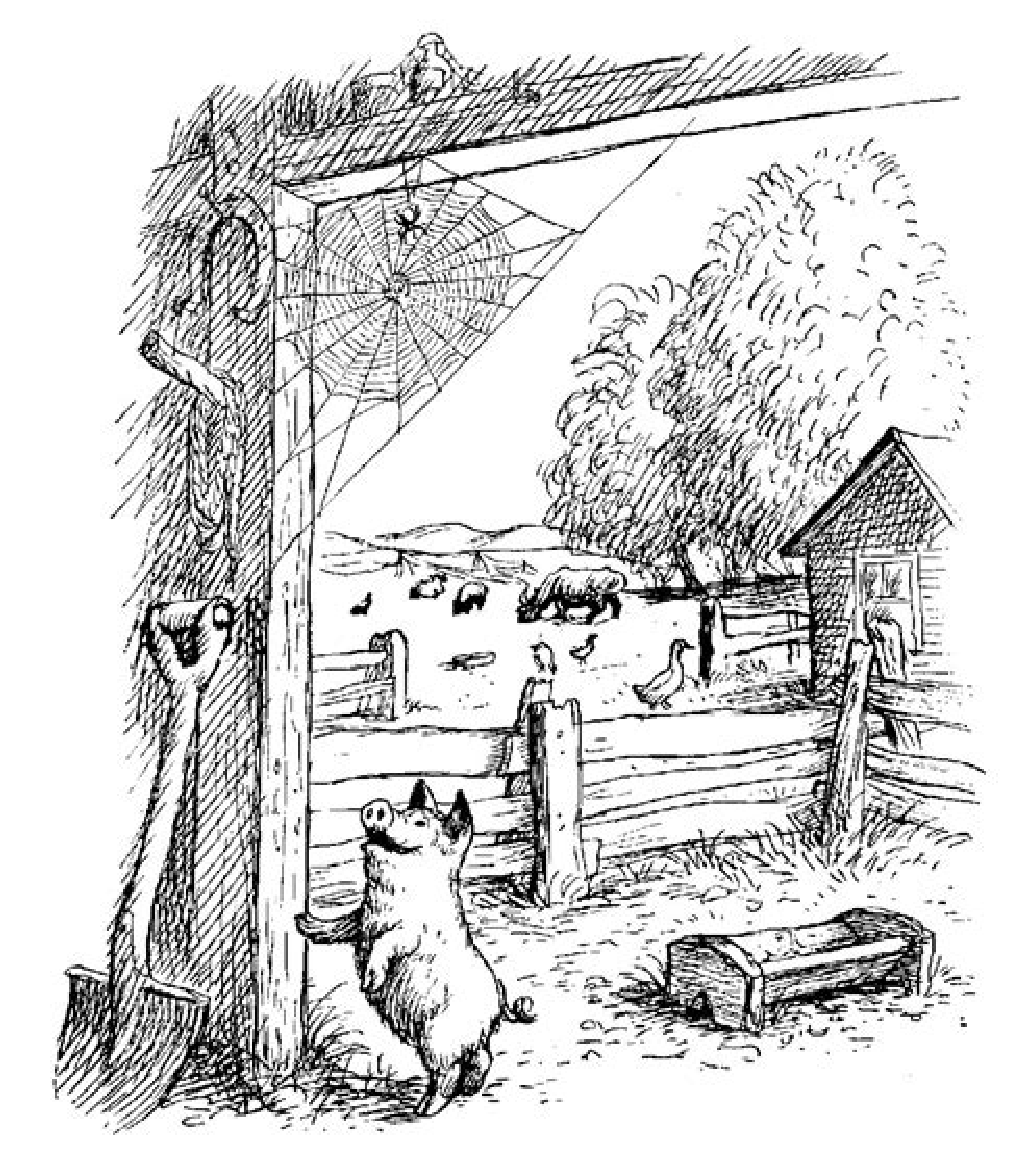
\includegraphics[scale=0.5]{cover.eps}
 
  \chapter{Bad News}
 Wilbur liked Charlotte better and better each day. Her campaign
against insects seemed sensible and useful. Hardly anybody 
around the farm had a good word to say for a fly. Flies spent their
time pestering others. The cows hated them. The horses detested
them. The sheep loathed them. Mr. and Mrs. Zukerman were
always complaining about them, and putting up screens.

 Wilbur admired the way Charlotte managed. He was particularly
glad that she always put her victim to sleep before eating it.

 ``It's real thoughtful of you to do that, Charlotte,'' he said.

 ``Yes,'' she replied in her sweet, musical voice, ``I always give them
an anaesthetic so they won't feel pain. It's a little service I throw
in.''

 As the days went by, Wilbur grew and grew. He ate three big
meals a day. He spent long hours lying on his side, half asleep,
dreaming pleasant dreams. He enjoyed good health and he gained
a lot of weight. One afternoon, when Fern was sitting on her stool,
the oldest sheep walked into the barn, and stopped to pay a call on
Wilbur.

 ``Hello!'' she said. ``Seems to me you're putting on weight.''

 ``Yes, I guess I am,'' replied Wilbur. ``At my age it's a good idea to
keep gaining.''

 ``Just the same, I don't envy you,'' said the old sheep.`` You know
why they're fattening you up, don't you?''

 ``No,'' said Wilbur. 

 ``Well, I don't like to spread bad news,'' said the sheep, ``but
they're fattening you up because they're going to kill you, that's
why.''

 ``They're going to what?'' screamed Wilbur. Fern grew rigid on her
stool.

 ``Kill you. Turn you into smoked bacon and ham,'' continued the
old sheep. ``Almost all young pigs get murdered by the farmer as
soon as the real cold weather sets in. There's regular conspiracy
around here to kill you at Christmastime. Everybody is in the
plog--Lurvy, Zuckerman, even John Arable.'' 

  ``Mr. Arable?'' sobbed Wilbur. ``Fern's father?''

 ``Certainly. When a pig is to be butchered, everybody helps. I'm an
old sheep and I see the same thing, same old business, year after
year. Arable arrives with hi .22, shoots the...''

 ``Stop!'' screamed Wilbur. ``I don't want to die! Save me, somebody!
Save me!'' Fern was just about to jump up when a voice was heard.

 ``Be quiet, Wilbur!'' said Charlotte, who had been listening to this
awful conversation.

 ``I can't be quiet,'' screamed Wilbur, racing up and down. ``I don't
want to be killed. I don't want to die. Is it true what the old sheep
says, Charlotte? Is it true they are going to kill me when the cold
weather comes?'' 

 ``Well,'' said the spider, plucking thoughtfully at her web, ``the old
sheep has been around this barn a long time. She has seen many a
spring pig come and go. If she says they plan to kill you, I'm sure
it's true. It's also the dirtiest trick I ever heard of. What people
don't think of!'' 

 Wilbur burst into tears. ``I don't want to die,'' he moaned. ``I want
to stay alive, right here in my comfortable manure pile with all my
friends. I want to breathe the beautiful air and lie in the beautiful
sun.''

 ``You're certainly making a beautiful noise,'' snapped the old sheep.

 ``I don't want to die!'' screamed Wilbur, throwing himself to the
ground.

 ``You shall not die,'' said Charlotte, briskly.

 ``What? Really?'' cried Wilbur. ``Who's going to save me?''

 ``I am,'' said Charlotte.

 ``How?'' asked Wilbur.

 ``That remains to be seen. But I am going to save you, and I want
you to quiet down immediately. You're carrying on in a childish
way. Stop your crying! I can't stand hysterics.'' 

  \chapter{A Talk at Home}
 On Sunday morning Mr. and Mrs. Arable and Fern were sitting at
breakfast in the kitchen. Avery had finished and was upstairs
looking for his slingshot.

 ``Did you know that Uncle Homer's goslings had hatched?'' asked
Fern.

 ``How many?'' asked Mr. Arable.

 ``Seven,'' replied Fern. ``There were eight eggs but one egg didn't
hatch and the goose told Templeton she didn't want it any more, so
he took it away.''

 ``The goose did what?'' asked Mrs. Arable, gazing at her daughter
with a queer, worried look.

 ``Told Templeton she didn't want the egg any more,'' repeated
Fern.

 ``Who is Templeton?'' asked Mrs. Arable.

 ``He's the rat,'' replied Fern. ``None of us like him much.''

 ``Who is 'us'?'' asked Mr. Arable.

 ``Oh, everybody in the barn cellar. Wilbur and the sheep and the
lambs and the goose and the gander and the goslings and Charlotte
and me.'' 

 ``Charlotte?'' said Mrs. Arable. ``Who's Charlotte?''

 ``She's Wilbur's best friend. She's terribly clever.''

 ``What does she look like?'' asked Mrs. Arable.

 ``Well-l,'' said Fern, thoughtfully,`` she has eight legs. All spiders
do, I guess.''

 ``Charlotte is a spider?'' asked Fern's mother.

 Fern nodded. ``A big grey one. She has a web across the top of
Wilbur's doorway. She catches flies and sucks their blood. Wilbur
adores her.''

 ``Does he really?'' said Mrs. Arable, rather vaguely. She was
staring at Fern with a worried expression on her face.

 ``Oh, yes, Wilbur adores Charlotte,'' said Fern. ``Do you know what
Charlotte said when the goslings hatched?''

 ``I haven't the faintest idea,'' said Mr. Arable. ``Tell us.''

 ``Well, when the first gosling stuck its little head out from under
the goose, I was sitting on my stool in the corner and Charlotte was
on her web. She made a speech.'' She said:`` I am sure that every one
of us here in the barn cellar will be gratified to learn that after four
weeks of unremitting effort and patience on the part of the goose,
she now has something to show for it.' Don't you think that was a
pleasant thing for her to say?''

 ``Yes, I do,'' said Mrs. Arable. ``And now, Fern, it's time to get 
 ready for Sunday School And tell Avery to get ready. And this
afternoon you can tell me more about what goes on in Uncle
Homer's barn. Aren't you spending quite a lot of time there? You
go there almost every afternoon, don't you?''

 ``I like it there,'' replied Fern. She wiped her mouth and ran
upstairs. After she had left the room, Mrs. Arable spoke in a low
voice to her husband.

 ``I worry about Fern,'' she said. ``Did you hear the way she rambled
on about the animals, pretending that they talked?''

 Mr. Arable chuckled. ``Maybe they do talk,'' he said. ``I've
sometimes wondered. At any rate, don't worry about Fern--she's
just got a lively imagination. Kids think they hear all sorts of
things.''

 ``Just the same, I do worry about her,'' replied Mrs. Arable. ``I
think I shall ask Dr. Dorian about her the next time I see him. He
loves Fern almost as much as we do, and I want him to know how
queerly she is acting about that pig and everything. I don't think
it's normal. You know perfectly well animals don't talk.''

 Mr. Arable grinned. ``Maybe our ears aren't as sharp as Fern's,'' he
said. 


  \chapter{Wilbur's Boast}
A spider's web is stronger than it looks. Although it is made of
thin, delicate strands, the web is not easily broken. However, a web
gets torn every day by the insects that kick around in it, and a
spider must rebuild it when it gets full of holes. Charlotte liked to
do her weaving during the late afternoon, and Fern liked to sit
nearby and watch. One afternoon she heard a most interesting
conversation and witnessed a strange event.

 ``You have awfully hairy legs, Charlotte,'' said Wilbur, as the
spider busily worked at her task.

 ``My legs are hairy for a good reason,'' replied Charlotte.
``Furthermore, each leg of mine has seven sections -- the coxa, the
trochanter, the femur, the patella, the tibia, the metatarsus, and
the tarsus.''

Wilbur sat bolt upright, ``You're kidding,'' he said.

 ``No, I'm not, either.''
 
 ``Say those names again, I didn't catch them the first time.''
 
 ``Coxa, trochanter, femur, patella, tibia, metatarsus, and tarsus.''
 
 ``Goodness!'' said Wilbur, looking down at his own chubby legs. ``I
don't think my legs have seven sections.''

 ``Well,'' said Charlotte, ``you and I lead different lives. You don't
have to spin a web. That takes real leg work.''

 ``I could spin a web if I tried,'' said Wilbur, boasting. ``I've just
never tried.''

``Let’s see you do it,'' said Charlotte. Fern chuckled softly,and her eyes grew wide with love for the pig.

``O.K.,'' replied Wilbur. ``You coach me and I'll spin one. Itmust be a lot of fun to spin a web. How do I start?''

``Take a deep breath!'' said Charlotte, smiling. Wilbur breatheddeeply.

``Now climb to the highest place you can get to, like this.''

Charlotte raced up to the top of the doorway. Wilbur scrambled to the top of the manure pile.

``Very good!'' said Charlotte. ``Now make an attachment with your
spinnerets, hurl yourself into space, and let out a dragline as you go
down!''

Wilbur hesitated a moment, then jumped out into the air. He
glanced hastily behind to see if a piece of rope was following him to
check his fall, but nothing seemed to be happening in his rear, and
the next thing he knew he landed with a thump. ``Ooomp!'' he
grunted.

 Charlotte laughed so hard her web began to sway. 

 ``What did I do wrong?'' asked the pig, when he recovered from
his bump.

 ``Nothing,'' said Charlotte. ``It was a nice try.'' 

 ``I think I’ll try again,'' said Wilbur, cheerfully. ``I believe what I
need is a little piece of string to hold me.''

 The pig walked out to his yard. ``You there, Templeton?'' he
called. The rat poked his head out from under the trough. 

``Got a little piece of string I could borrow?'' asked Wilbur. ``I
need it to spin a web.''

 ``Yes, indeed,'' replied Templeton, who saved string. ``No
trouble at all. Any thing to oblige.'' He crept down into his hole,
pushed the goose egg out of the way, and returned with an old
piece of dirty white string. Wilbur examined it.

 ``That’s just the thin,'' he said. ``Tie one end to my tail, will you,
Templeton?''

Wilbur crouched low, with his thin, curly tail toward the rat.
Templeton seized the string, passed it around the end of the pig's
tail, and tied two half hitches. Charlotte watched in delight. Like
Fern, she was truly fond of Wilbur, whose smelly pen and stale
food attracted the flies that she needed, and she was proud to see
that he was not a quitter and was willing to try again to spin a web.

 While the rat and the spider and the little girl watched, Wilbur
climbed again to the top of the manure pile, full of energy and hope. 

``Everybody watch!'' he cried. And summoning all his strength, 
he threw himself into the air, headfirst. The string trailed behind
him. But as he had neglected to fasten the other end to anything, it
didn't really do any good, and Wilbur landed with a thud, crushed
and hurt. Tears came to his eyes. Templeton grinned. Charlotte
just sat quietly. After a bit she spoke. 

``You can’t spin a web, Wilbur, and I advise you to put the idea
out of your mind. You lack two things needed for spinning a web.''

``What are they?'' asked Wilbur, sadly.

``You lack a set of spinnerets, and you lack know-how. But
cheer up, you don't need a web. Zucherman supplies you with three
big meals a day. Why should you worry about trapping food?''

Wilbur sighed. ``You're ever so much cleverer and brighter
than I am, Charlotte. I guess I was just trying to show off. Serves
me right.'' 

Templeton untied his string and took it back to his home. Charlotte
returned to her weaving.

``You needn't feel too badly, Wilbur,'' she said. ``Not many
creatures can spin webs. Even men aren't as good at it as spiders,
although they think they're pretty good, and they'll try anything.
Did you ever hear of the Queensborough Bridge?''

Wilbur shook his head. ``Is it a web?'' 

``Sort of,'' replied Charlotte. ``But do you know how long it took 
men to build it? Eight whole years. My goodness, I would have
starved to death waiting that long. I can make a web in a single
evening.''

``What do people catch in the Queensborough Bridge—bug?''
asked Wilbur. 

``No,'' said Charlotte. ``They don’t catch anything. They just
keep trotting back and forth across the bridge thinking there is
something better on the other side. If they’d hang head-down at
the top of the thing and wait quietly, maybe something good would
come along. But no—with men it’s rush, rush, rush, every minute.
I’m glad I’m a sedentary spider.''

``What does sedentary mean?'' asked Wilbur.

``Means I sit still a good part of the time and don’t go
wandering all over creation. I know a good thing when I see it, and
my web is a good thing. I stay put and wait for what comes. Gives
me a chance to think.'' 

``Well, I’m sort of sedentary myself, I guess,'' said the pig. ``I
have to hang around here whether I want to or not. You know
where I'd really like to be this evening?''

``Where?''

``In a forest looking for beechnuts and truffles and delectable
roots, pushing leaves aside with my wonderful strong nose,
searching and sniffing along the ground, smelling, smelling,
smelling…''

``You smell just the way you are,'' remarked a lamb who had
just walked in. ``I can smell you from here. You're the smelliest
creature in the place.''

Wilbur hung his head. His eyes grew wet with tears. Charlotte
noticed his embarrassment and she spoke sharply to the lamb.

 ``Leave Wilbur alone!'' she said. ``he has a perfect right to smell,
considering his surroundings. You're no bundle of sweet peas
yourself. Furthermore, you are interrupting a very pleasant
conversation. What were we talking about, Wilbur, when we were
so rudely interrupted?'' 

``Oh, I don't remember,'' said Wilbur. ``It doesn't make any
difference.. Let's not talk any more for a while, Charlotte. I'm
getting sleepy. You go ahead and finish fixing your web and I'll just
lie here and watch you. It's a lovely evening.'' Wilbur stretched out
on his side.

 Twilight settled over Zuckerman's barn, and a feeling of peace.
Fern knew it was almost suppertime but she couldn't bear to leave.
Swallows passed on silent wings, in and out of the doorways,
bringing food to their young ones. From across the road a bird sang

``Whippoorwill, whippoorwill!'' Lurvy sat down under and apple 
tree and lit his pipe; the animals sniffed the familiar smell of strong
tobacco. Wilbur heard the trill of the tree toad and the occasional
slamming of the kitchen door. All these sounds made him feel
comfortable and happy, for he loved life and loved to be a part of
the world on a summer evening. But as he lay there he
remembered what the old sheep had told him. The thought of
death came to him and he began to tremble with fear. 

``Charlotte?'' he said, softly.

 ``Yes, Wilbur?''

 ``I don’t want to die.''

 ``Of course you don’t,'' said Charlotte in a comforting voice.

 ``I just love it here in the barn,'' said Wilbur. ``I love everything
about this place.''

 ``Of course you do,'' said Charlotte. ``We all do.''

 The goose appeared, followed by her seven goslings. They
thrust their little necks out and kept up a musical whistling, like a
tiny troupe of pipers. Wilbur listened to the sound with love in his
heart. 

``Charlotte?'' he said.

 ``Yes?'' said the spider.

 ``Were you serious when you promised you would keep them
from killing me?'' 

``I was never more serious in my life. I am not going to let you
die, Wilbur.''

 ``How are you going to save me?'' asked Wilbur, whose
curiosity was very strong on this point.

 ``Well,'' said Charlotte, vaguely, ``I don't really know. But I'm
working on a plan.''

 `` That's wonderful,'' said Wilbur. ``How is the plan coming,
Charlotte? Have you got very far with it? Is it coming along pretty
well?'' Wilbur was trembling again, but Charlotte was cool and
collected.

 ``Oh, it's coming all right,'' she said, lightly. ``The plan is still in
its early stages had hasn't completely shaped up yet, but I'm
working on it. ''

``When do you work on it?'' begged Wilbur.

 ``When I'm hanging head-down at the top of my web. That’s
when I do my thinking, because then all the blood is in my head.''

 ``I'd be only too glad to help in any way I can.''

 ``Oh, I'll work it out alone,'' said Charlotte. ``I can think better if
I think alone.''

 ``All right,'' said Wilbur. ``But don't fail to let me know if there's
anything I can do to help, no matter how slight.''

``Well,'' replied Charlotte, ``you must try to build yourself up. I
 want you to get plenty of sleep, and stop worrying. Never hurry and
never worry! Chew your food thoroughly and eat every bit of it,
except you must leave just enough for Templeton. Gain weight and
stay well—that’s the way you can help. Keep fit, and don’t lose your
nerve. Do you think you understand?''

``Yes, I understand,'' said Wilbur.

``Go along to bed, then,'' said Charlotte. ``Sleep is important.''

Wilbur trotted over to the darkest corner of his pen and threw
himself down. He closed his eyes. In another minute he spoke. 

``Charlotte?'' he said.

``Yes, Wilbur?''

``May I go out to my trough and see if I left any of my supper? I
think I left just a tiny bit of mashed potato.''

``Very well,'' said Charlotte. ``But I want you in bed again
without delay.''

Wilbur started to race out to his yard.

``Slowly, slowly!'' said Charlotte. ``Never hurry and never
worry!''

 Wilbur checked himself and crept slowly to his trough. He
found a bit of potato, chewed it carefully, swallowed it, and walked
back to bed. He closed his eyes and was silent for a while.

 ``Charlotte?'' he said, in a whisper. 

 ``Yes?''

 ``May I get a drink of milk? I think there are a few drops of
milk left in my trough.''

 ``No, the trough is dry, and I want you to go to sleep. No more
talking! Close your eyes and go to sleep!''

 Wilbur shut his eyes. Fern got up from her stool and started
for home, her mind full of everything she had seen and heard.

 ``Good night, Charlotte!'' said Wilbur.

 ``Good night, Wilbur!''
 There was a pause.

 ``Good night, Charlotte!''

 ``Good night, Wilbur!''

 ``Good night!''

 ``Good night!''
 
 \chapter{An Explosion}
 Day after day the spider waited, head-down, for an idea to come
to her. Hour by hour she sat motionless, deep in thought. Having
promised Wilbur that she would save his life, she was determined 
to keep her promise. 

Charlotte was naturally patient. She knew from experience
that if she waited long enough, a fly would come to her web; and
she felt sure that if she thought long enough about Wilbur¡¯s
problem, and idea would come to her mind.
 Finally, one morning toward the middle of July, the idea came.

``Why, how perfectly simple!'' she said to herself. ``The way to save
Wilbur's life is to play a trick on Zuckerman. If I can fool a bug,''
thought Charlotte, ``I can surely fool a man. People are not as smart
as bugs.''

Wilbur walked into his yard just at that moment.

``What are you thinking about, Charlotte?'' he asked.

``I was just thinking,'' said the spider, ``that people are very
gullible.''

``What does 'gullible' mean?''

``Easy to fool,'' said Charlotte.

``That's a mercy,'' replied Wilbur, and he lay down in the shade
of his fence and went fast asleep. The spider, however, stayed wide
awake, gazing affectionately at him and making plans for his future. 
Summer was half gone. She knew she didn't have much time.

 That morning, just as Wilbur fell asleep, Avery Arable
wandered into the Zuckerman's front yard, followed by Fern. Avery
carried a live frog in his hand. Fern had a crown of daisies in her
hair. The children ran for the kitchen. 

``Just in time for a piece of blueberry pie,'' said Mrs.
Zuckerman.

``Look at my frog!'' said Avery, placing the frog on the
drainboard and holding out his hand for pie.

``Take that thing out of here!'' said Mrs. Zuckerman.

``He's hot,'' said Fern. ``He's almost dead, that frog.'' 

``He is not,'' said Avery. ``He lets me scratch him between the
eyes.'' The frog jumped and landed in Mrs. Zuckerman's dishpan
full of soapy water.

``You're getting your pie on you,'' said Fern. ``Can I look for
eggs in the henhouse, Aunt Edith?''

``Run outdoors, both of you! And don't bother the hens!''

``It's getting all over everything,'' shouted Fern. ``His pie is all
over his front.''

``Come on, frog!'' cried Avery. He scooped up his frog. The fog
kicked, splashing soapy water onto the blueberry pie.

``Another crisis!'' groaned Fern. 

``Let's swing in the swing!'' said Avery. 

The children ran to the barn.

 Mr. Zuckerman had the best swing in the county. It was a
single long piece of heavy rope tied to the beam over the north
doorway. At the bottom end of the rope was a fat knot to sit on. It
was arranged so that you could swing without being pushed. You
climbed a ladder to the hayloft. Then, holding the rope, you stood
at the edge and looked down, and were scared and dizzy. Then you
straddled the knot, so that it acted as a seat. Then you got up all
your nerve, took a deep breath, and jumped. For a second you
seemed to be falling to the barn floor far below, but then suddenly
the rope would begin to catch you, and you would sail through the
barn door going a mile a minute, with the wind whistling in your
eyes and ears and hair. Then you would zoom upward into the sky, 
and look up at the clouds, and the rope would twist and you would
twist and turn with the rope. Then you would drop down, down,
down out of the sky and come sailing back into the barn almost
into the hayloft, then sail out again (not quite so far this time), then
in again (not quite so high), then out again, then in again, then out,
then in; and then you'd jump off and fall down and let somebody
else try it. 

Mothers for miles around worried about Zuckerman's swing.
They feared some child would fall off. But no child ever did.
Children almost always hang onto things tighter than their parents
think they will.

 Avery put the frog in his pocket and climbed to the hayloft.
``The last time I swang in this swing, I almost crashed into a barn
swallow,'' he yelled. 

``Take that frog out!'' ordered Fern.

Avery straddled the rope and jumped. He sailed out through
the door, frog and all, and into the sky, frog and all. Then he sailed
back into the barn.

``Your tongue is purple!'' screamed Fern.

``So is yours!'' cried Avery, sailing out again with the frog.

``I have hay inside my dress! It itches!'' called Fern.

``Scratch it!'' yelled Avery, as he sailed back.

``It's my turn,'' said Fern. ``Jump off!''

``Fern's got the itch.'' sang Avery.

When he jumped off, he threw the swing up to his sister. She
shut her eyes tight and jumped. She felt the dizzy drop, then the
supporting lift of the swing. When she opened her eyes she was
looking up into the blue sky and was about to fly back through the
door.

They took turns for and hour.

When the children grew tired of swinging, they went down
toward the pasture and picked wild raspberries and ate them. Their
tongues turned from purple to red. Fern bit into a raspberry that
had a bad-tasting bug inside it, and got discouraged. Avery found
and empty candy box and put his frog in it. The frog seemed tired
after his morning in the swing. The children walked slowly up
toward the barn. They, too, were tired and hardly had energy
enough to walk.

``Let's build a tree house,'' suggested Avery. ``I want to live in a
tree, with my frog.''

``I'm going to visit Wilbur,'' Fern announced.

They climbed the fence into the lane and walked lazily toward
the pigpen. Wilbur heard them coming and got up.

Avery noticed the spider web, and , coming closer, he saw
Charlotte.

``Hey, look at that big spider!'' he said. ``It's tremendous.''

``Leave it alone!'' commanded Fern. ``You've got a frog---isn't
that enough?''

``That's a fine spider and I'm going to capture it,'' said Avery.

He took the cover off the candy box. Then he picked up a stick. ``I'm
going to knock that old spider into this box,'' he said.

Wilbur's heart almost stopped when he saw what was going on.
This might be the end of Charlotte if the boy succeeded in catching
her.

``You stop it, Avery!'' cried Fern.

Avery put one leg over the fence of the pigpen. He was just
about to raise his stick to hit Charlotte when he lost his balance. He
swayed and toppled and landed on the edge of Wilbur¡¯s trough.
The trough tipped up and then came down with a slap. The goose
egg was right underneath. There was a dull explosion as the egg
broke, and then a horrible smell.

Fern screamed. Avery jumped to his feet. The air was filled
with the terrible gases and smells from the rotten egg. Templeton,
who had been resting in his home, scuttled away into the barn.

``Good night!'' screamed Avery. ``Good night! What a stink!
Let's get out of here!''

Fern was crying. She held her nose and ran toward the house.
Avery ran after her, holding his nose. Charlotte felt greatly relieved
to see him go. It had been a narrow escape.

Later on that morning, the animals came up from the
pasture---the sheep, the lambs, the gander, the goose, and the
seven goslings. There were many complaints about the awful smell,
and Wilbur had to tell the story over and over again, of how the
Arable boy had tried to capture Charlotte, and how the smell of the
broken egg drove him away just in time. ``It was that rotten goose
egg that saved charlotte's life,'' said Wilbur.

The goose was proud of her share in the adventure. ``I'm
delighted that the egg never hatched,'' she gabbled.

Templeton, of course, was miserable over the loss of his
beloved egg. But he couldn't resist boasting. ``It pays to save
things,'' he said in his surly voice. ``A rat never knows when
something is going to come in handy. I never throw anything away.''

``Well,'' said one of the lambs, ``this whole business is all well
and good for Charlotte, but what about the rest of us? The smell is
unbearable. Who wants to live in a barn that is perfumed with
rotten egg?''

``Don't worry, you'll get used to it,'' said Templeton. He sat up
and pulled wisely at his long whiskers, then crept away to pay a
visit to the dump.

When Lurvy showed up at lunchtime carrying a pail of food for
Wilbur, he stopped short a few paces from the pigpen. He sniffed
the air and made a face.

``What in thunder?'' he said. Setting the pail down, he picked
up the stick that Avery had dropped and pried the trough up.
``Rats!'' he said. ``Phew! I might know a rat would make a nest
under this trough. How I hate a rat!''

And Lurvy dragged Wilbur's trough across the yard and kicked
some dirt into the rat's nest, burying the broken egg and all
Templeton's other possessions. Then he picked up the pail. Wilbur
stood in the trough, drooling with hunger. Lurvy poured. The slops
ran creamily down around the pig's eyes and ears. Wilbur grunted.
He gulped and sucked, making swishing and swooshing noises,
anxious to get everything at once. It was a delicious meal¡ªskim
milk, wheat middlings, leftover pancakes, half a doughnut, the rind
of a summer squash, two pieces of stale toast, a third of a
gingersnap, a fish tail, one orange peel, several noodles from a
noodle soup, the scum off a cup of cocoa, an ancient jelly roll, a
strip of paper from the lining of the garbage pail, and a spoonful of
raspberry jello.

Wilbur ate heartily. He planned to leave half a noodle and a
few drops of milk for Templeton. Then he remembered that the rat
had been useful in saving Charlotte's life, and that Charlotte was             \marginpar{save sb's life}
trying to save his life. So he left a whole noodle, instead of a half.

Now that the broken egg was buried, the air cleared and the
barn smelled good again. The afternoon passed, and evening came.
Shadows lengthened. The cool and kindly breath of evening
entered through doors and windows. Astride her web, Charlotte sat
moodily eating a horsefly and thinking about the future. After a
while she bestirred herself.

She descended to the center of the web and there she began to
cut some of her lines. She worked slowly but steadily while the
other creatures drowsed. None of the others, not even the goose,
noticed that she was at work. Deep in his soft bed, Wilbur snoozed.
Over in their favorite corner, the goslings whistled a night song.

Charlotte tore quite a section out of her web, leaving an open
space in the middle. Then she started weaving something to take
the place of the threads she had removed. When Templeton got
back from the dump, around midnight, the spider was still at work.

  \chapter{The Miracle}

The next day was foggy. Everything on the farm was dripping wet.
The grass looked like a magic carpet. The asparagus patch looked
like a silver forest.

On foggy mornings, Charlotte's web was truly a thing of beauty.
This morning each thin strand was decorated with dozens of tiny
beads of water. The web glistened in the light and made a pattern
of loveliness and mystery, like a delicate veil. Even Lurvy, who
wasn't particularly interested in beauty, noticed the web when he
came with the pig's breakfast. He noted how clearly it showed up
and he noted how big and carefully built it was. And then he took
another look and he saw something that made him set his pail
down. There, in the center of the web, neatly woven in block letters,
was a message. It said: SOME PIG!                                                \marginpar{\underline{some} here means \textit{awesome, perfect}}

Lurvy felt weak. He brushed his hand across his eyes and
stared harder at Charlotte's web. ``I'm seeing things,'' he whispered.

He dropped to his knees and uttered a short prayer. Then,
forgetting all about Wilbur's breakfast, he walked back to the house
and called Mr. Zuckerman.

``I think you'd better come down to the pigpen,'' he said.

``What's the trouble?'' asked Mr. Zuckerman. ``Anything wrong
with the pig?''

``N-not exactly,'' said Lurvy. ``Come and see for yourself.''
The two men walked silently down to Wilbur's yard. Lurvy
pointed to the spider's web. ``Do you see what I see?'' he asked.

Zuckerman stared at the writing on the web. Then he
murmured the words ``Some Pig.'' Then he looked at Lurvy. Then
they both began to tremble. Charlotte, sleepy after her night's
exertions, smiled as she watched. Wilbur came and stood directly
under the web.

``Some pig!'' muttered Lurvy in a low voice.

``Some pig!'' Whispered Mr. Zuckerman. They stared and
stared for a long time at Wilbur. Then they stared at Charlotte.

``You don't suppose that that spider . . . '' began Mr.
Zuckerman---but he shook his head and didn't finish the sentence.
Instead, he walked solemnly back up to the house and spoke to his
wife. ``Edith, something has happened,'' he said, in a weak voice.
He went into the living room and sat down and Mrs. Zuckerman
followed.

``I've got something to tell you, Edith,'' he said. ``You better sit
down.''

Mrs. Zuckerman sank into a chair. She looked pale and frightened.
``Edith,'' he said, trying to keep his voice steady, ``I think you
had best be told that we have a very unusual pig.''
A look of complete bewilderment came over Mrs. Zuckerman's
face. ``Homer Zuckerman, what in the world are you talking
about?'' she said.

``This is a very serious thing, Edith,'' he replied.

``Our pig is completely out of the ordinary.''

``What's unusual about the pig?'' asked Mrs. Zuckerman, who
was beginning to recover from her scare.

``Well, I don't really know yet,'' said Mr. Zuckerman. ``But we
have received a sign, Edith---a mysterious sign. A miracle has
happened on this farm. There is a large spider's web in the
doorway of the barn cellar, right over the pigpen, and when Lurvy
went to feed the pig this morning, he noticed the web because it
was foggy, and you know how a spider's web looks very distinct in a
fog. And right spang in the middle of the web there were the words
'Some Pig.' The words were woven right into the web. They were
actually part of the web, Edith. I know, because I have been down
there and seen them. It says, 'Some Pig,' just as clear as clear can
be. There can be no mistake about it. A miracle has happened and
a sign has occurred hereon earths right on our farm, and we have
no ordinary pig.''

``Well,'' said Mrs. Zuckerman, ``it seems to me you're a little off.
It seems to me we have no ordinary spider.''

``Oh, no,'' said Zuckerman. ``It's the pig that's unusual. It says
so, right there in the middle of the web.''

``Maybe so,'' said Mrs. Zuckerman. ``Just the same, I intend to
have a look at that spider.''

``It's just a common grey spider,'' said Zuckerman.
They got up, and together they walked down to Wilbur's yard.

``You see, Edith? It's just a common grey spider.''

Wilbur was pleased to receive so much attention. Lurvy was
still standing there, and Mr. And Mrs. Zuckerman, all three, stood
for about an hour, reading the words on the web over and over, and
watching Wilbur.

Charlotte was delighted with the way her trick was working.
She sat without moving a muscle, and listened to the conversation
of the people. When a small fly blundered into the web, just beyond
the word ``pig,'' Charlotte dropped quickly down, rolled the fly up,
and carried it out of the way.

After a while the fog lifted. The web dried off and the words
didn't show up so plainly. The Zuckermans and Lurvy walked back
to the house. Just before they left the pigpen, Mr. Zuckerman took
one last look at Wilbur.

``You know,'' he said, in an important voice, ``I've thought all
along that that pig of ours was an extra good one. He¡¯s a solid pig.
That pig is as solid as they come. You notice how solid he is around
the shoulders, Lurvy?''

``Sure, Sure I do,'' said Lurvy. ``I've always noticed that pig.
He's quite a pig.''

``He's long, and he's smooth,'' said Zuckerman.

``That's right,'' agreed Lurvy. ``he's as smooth as they come.
He's some pig.''

When Mr. Zuckerman got back to the house, he took off his
work clothes and put on his best suit. Then he got into his car and
drove to the minister¡¯s house. He stayed for an hour and explained
to the minister that a miracle had happened on the farm.

``So far,'' said Zuckerman, ``only four people on earth know
about this miracle --- myself, my wife Edith, my hired man Lurvy,
and you.''

``Don't tell anybody else,'' said the minister. ``We don't know
what it means yet, but perhaps if I give thought to it, I can explain
it in my sermon next Sunday. There can be no doubt that you have
a most unusual pig. I intend to speak about it in my sermon and
point out the fact that this community has been visited with a
wondrous animal. By the way, does the pig have a name?''

``Why, yes,'' said Mr. Zuckerman. ``My little niece calls him
Wilbur. She's rather queer child---full of notions. She raised the pig
on a bottle and I bought him from her when he was a month old.''

He shook hands with the minister, and left.

Secrets are hard to keep. Long before Sunday came, the news
spread all over the county. Everybody knew that a sign had
appeared in a spider's web on the Zuckerman place. Everybody
knew that the Zuckermans had a wondrous pig. People came from
miles around to look at Wilbur and to read the words on
Charlotte¡¯s web. The Zuckermans' driveway was full of cars and
trucks from morning till night--Fords and Chevvies and Buick
roadmasters and GMC pickups and Plymouths and Studebakers
and Packards and De Sotos with gyromatic transmissions and
Oldsmobiles with rocket engines and Jeep station wagons and
Pontiacs. The news of the wonderful pig spread clear up into the
hills, and farmers came rattling down in buggies and buckboards,
to stand hour after hour at Wilbur's pen admiring the miraculous
animal. All said they had never seen such a pig before in their lives.

When Fern told her mother that Avery had tried to hit the
Zuckermans' spider with a stick, Mrs. Arable was so shocked that
she sent Avery to bed without any supper, as punishment.

In the days that followed, Mr. Zuckerman was so busy
entertaining visitors that he neglected his farm work. He wore his
good clothes all the time now---got right into them when he got up
in the morning. Mrs. Zuckerman prepared special meals for Wilbur.
Lurvy shaved and got a haircut; and his principal farm duty was to
feed the pig while people looked on.

Mr. Zuckerman ordered Lurvy to increase Wilbur's feedings
from three meals a day to four meals a day. The Zuckermans were
so busy with visitors they forgot about other things on the farm.
The blackberries got ripe, and Mrs. Zuckerman failed to put up any
blackberry jam. The corn needed hoeing, and Lurvy didn't find
time to hoe it.

On Sunday the church was full. The minister explained the
miracle. He said that the words on the spider's web proved that
human beings must always be on the watch for the coming of
wonders.

All in all, the Zuckermans' pigpen was the center of attraction.
Fern was happy, for she felt that Charlotte's trick was working and
that Wilbur's life would be saved. But she found that the barn was
not nearly as pleasant---too many people. She liked it better when
she could be all alone with her friends the animals.


 \chapter{A Metting}
 
One evening, a few days after the writing had appeared in

Charlotte's web, the spider called a meeting of all the animals in
the barn cellar.

``I shall begin by calling the roll. Wilbur?''

``Here!'' said the pig.

``Gander?''

``Here, here, here!'' said the gander.

``You sound like three ganders,'' muttered Charlotte. ``Why can't
you just say 'here'? Why do you have to repeat everything?''

``It's my idio-idio-idiosyncrasy,'' replied the gander.

``Goose?'' said Charlotte.

``Here, here, here!'' said the goose. Charlotte glared at her.

``Goslings, one through seven?''

``Bee-bee-bee!'' ``Bee-bee-bee!'' ``Bee-bee-bee!'' ``Bee-bee-bee!''

``Bee-bee-bee!'' ``Bee-bee-bee!'' ``Bee-bee-bee!'' said the goslings.

``This is getting to be quite a meeting,'' said Charlotte. ``Any body
would think we had three ganders, three geese, and twenty-one
goslings. Sheep?''

``He-aa-aa!'' answered the sheep all together.

``Lambs?''

``He-aa-aa!'' answered the lambs all together.

``Templeton?''

No answer.

``Templeton?''

No answer.

``Well, we are all here except the rat,'' said Charlotte. ``I guess we
can proceed without him. Now, all of you must have noticed what's
been going on around here the last few days. The message I wrote
in my web, praising Wilbur, has been received. The Zuckermans
have fallen for it, and so has everybody else. Zuckerman thinks
Wilbur is an unusual pig, and therefore he won't want to kill him
and eat him. I dare say my trick will work and Wilbur's life can be
saved.''

``Hurray!'' cried everybody.

``Thank you very much,'' said Charlotte. ``Now I called this
meeting in order to get suggestions. I need new ideas for the web.
People are already getting sick of reading the words 'Some Pig!' If
anybody can think of another message, or remark, I'll be glad to
weave it into the web. Any suggestions for a new slogan?''

``How about 'Pig Supreme'?'' asked one of the lambs.

``No good,'' said Charlotte. ``It sounds like a rich dessert.''

``How about 'Terrific, terrific, terrific'?'' asked the goose.

``Cut that down to one 'terrific' and it will do very nicely,'' said
Charlotte. ``I think 'terrific' might impress Zuckerman.''

``But Charlotte,'' said Wilbur, ``I'm not terrific.''

``that doesn't make a particle of difference,'' replied Charlotte.

``Not a particle. People believe almost anything they see in print.
Does anybody here know how to spell 'terrific'?''

``I think,'' said the gander,`` it's tee double ee double rr double rr
double eye double ff double eye double see see see see see.''

``What kind of an acrobat do you think I am?'' said Charlotte in
disgust. ``I would have to have St. Vitus's Dance to weave a word
like that into my web.''

``Sorry, sorry, sorry,'' said the gander.

Then the oldest sheep spoke up. ``I agree that there should be
something new written in the web if Wilbur's life is to be saved.
And if Charlotte needs help in finding words, I think she can get it
from our friend Templeton. The rat visits the dump regularly and
has access to old magazines. He can tear out bits of advertisements
and bring them up here to the barn cellar, so that Charlotte can
have something to copy.''

``Good idea,'' said Charlotte. ``But I'm not sure Templeton will be
willing to help. You know how he is--always looking out for himself,
never thinking of the other fellow.''

``I be I can get him to help,'' said the old sheep. ``I'll appeal to his
baser instincts, of which he has plenty. Here he comes now.
Everybody keep quiet while I put the matter up to him!''

The rat entered the barn the way he always did---creeping along
close to the wall.

``What's up?'' he asked, seeing the animals assembled.

``We're holding a directors' meeting,'' replied the old sheep.

``Well, break it up!'' said Templeton. ``Meetings bore me.'' And the
rat began to climb a rope that hung against the wall.

``Look,'' said the old sheep, ``next time you go to the dump,
Templeton, bring back a clipping from a magazine. Charlotte needs
new ideas so she can write messages in her web and save Wilbur's
life.''

``Let him die,'' said the rat. ``I should worry.''

``You'll worry all right when next winter comes,'' said the sheep.

``You'll worry all right on a zero morning next January when
Wilbur is dead and nobody comes down here with a nice pail of
warm slops to pour into the trough. Wilbur's leftover food is your
chief source of supply, Templeton. You know that. Wilbur's food is
your food; therefore Wilbur's destiny and you destiny are closely
linked. If Wilbur is killed and his trough stands empty day after
day, you'll grow so thin we can look right through your stomach
and see objects on the other side.''

Templeton's whiskers quivered.

``Maybe you're right,'' he said gruffly. ``I'm making a trip to the
dump tomorrow afternoon. I'll bring back a magazine clipping if I
can find one.''

``Thanks,'' said Charlotte. ``The meeting is now adjourned. I have a
busy evening ahead of me. I've got to tear my web apart and write
'Terrific.'''

Wilbur blushed. ``But I'm not terrific, Charlotte. I'm just about
average for a pig.''

``You're terrific as far as I'm concerned,'' replied Charlotte, sweetly,
``and that's what counts. You're my best friend, and I think you're
sensational. Now stop arguing and go get some sleep!''


 \chapter{Good Progress}
Far into the night, while the other creatures slept, Charlotte
worked on her web. First she ripped out a few of the orb lines near
the center. She left the radial lines alone, as they were needed for
support. As she worked, her eight legs were a great help to her. So
were her teeth. She loved to weave and she was an expert at it.
When she was finished ripping things out, her web looked
something like this:



 


\end{document}







